% первая глава

\section{Название первого раздела}

\subsection{Таблицы}

Текст подраздела посвящен таблице~\ref{tab:t1}

\begin{table}[H]
\caption{Пример таблицы}
\label{tab:t1}
\begin{center}
\begin{tabular}{|r|p{5.5cm}|p{2.5cm}|}
\hline 
1 & Первый текст в ячейке фиксированной ширины & $E=mc^2 $ \\ 
\hline 
12 & Второй текст тоже может быть произвольно длинным & $\sin \pi = 0 $ \\ 
\hline 
\end{tabular} 
\end{center}
\end{table}

\subsection{Вставка изображения}

\begin{figure}[H]
	\centering
	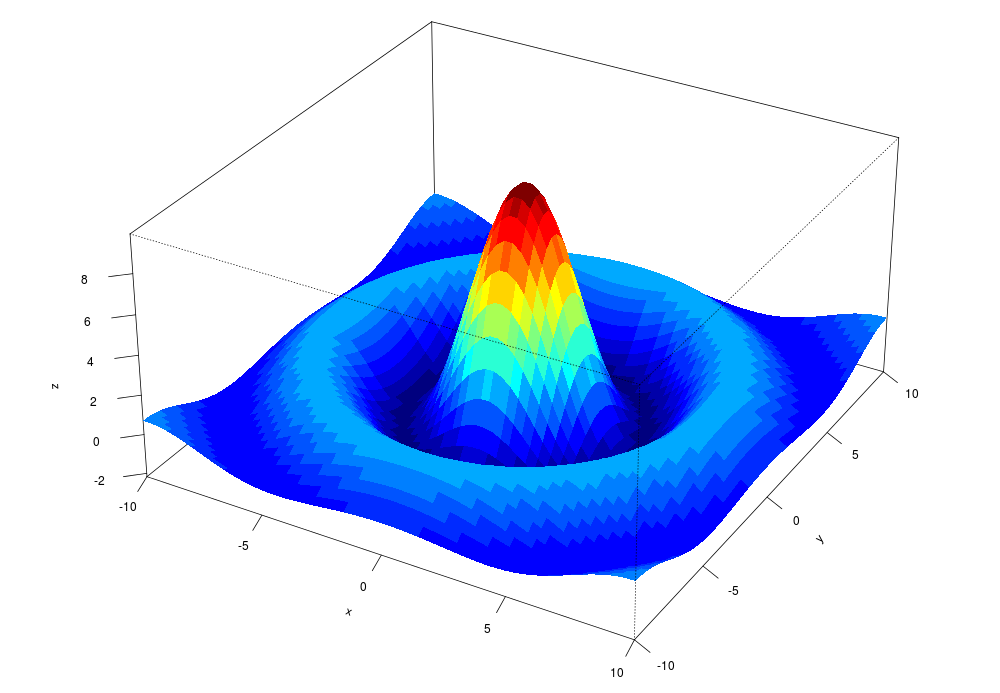
\includegraphics[width=0.7\linewidth]{pics/pic3D}
	\caption{Пример изображения для демонстрации возможности вставки в документ}
	\label{fig:pic3d}
\end{figure}



Изображение на рис.~\ref{fig:pic3d} находится в подкаталоге pics.

